\chapter{Debug Module (DM)} \label{dm}

\begin{steps}{The Debug Module implements a translation interface between abstract debug
    operations and their specific implementation. It might support the following
    operations:}
\item Give the debugger necessary information about the implementation. (Required)
\item Allow any individual hart to be halted and resumed. (Required)
\item Provide status on which harts are halted. (Required)
\item Provide abstract read and write access to a halted hart's GPRs. (Required)
\item Provide access to a reset signal that allows debugging from the very
    first instruction after reset. (Required)
\item Provide a mechanism to allow debugging harts immediately out of reset
      (regardless of the reset cause). (Optional)
\item Provide abstract access to non-GPR hart registers. (Optional)
\item Provide a Program Buffer to force the hart to execute arbitrary instructions. (Optional)
\item Allow multiple harts to be halted, resumed, and/or reset at the same time. (Optional)
\item Allow memory access from a hart's point of view. (Optional)
\item Allow direct System Bus Access. (Optional)
\item Group harts. When any hart in the group halts, they all halt. (Optional)
\item Respond to external triggers by halting each hart in a configured group. (Optional)
\item Signal an external trigger when a hart in a group halts. (Optional)
\end{steps}

\begin{steps}{In order to be compliant with this specification an
    implementation must:}
\item Implement all the required features listed above.
\item Implement at least one of Program Buffer, System Bus Access, or Abstract
    Access Memory command mechanisms.
\item
    \begin{steps}{Do at least one of:}
        \item Implement the Program Buffer.
        \item Implement abstract access to all registers that are visible to
            software running on the hart including all the registers that are
            present on the hart and listed in Table~\ref{tab:regno}.
        \item Implement abstract access to at least all GPRs, \Rdcsr, and
            \Rdpc, and advertise the implementation as conforming to the
            ``Minimal RISC-V Debug Specification \versionnum'', instead of the
            ``RISC-V Debug Specification \versionnum''.
    \end{steps}
\end{steps}

A single DM can debug up to $2^{20}$ harts.

\section{Debug Module Interface (DMI)} \label{dmi}

Debug Modules are slaves to a bus called the Debug Module Interface (DMI). The
master of the bus is the Debug Transport Module(s).
The Debug Module Interface can be a trivial bus with one master and one slave,
or use a more full-featured bus like TileLink or the AMBA Advanced Peripheral
Bus. The details are left to the system designer.

The DMI uses between 7 and 32 address bits.  It supports read and write
operations.  The bottom of the address space is
used for the first (and usually only) DM. Extra space can be used for custom
debug devices, other cores, additional DMs, etc. If there are additional DMs
on this DMI, the base address of the next DM in the DMI address space is given
in \Rnextdm.


The Debug Module is controlled via register accesses to its DMI address space.

\section{Reset Control} \label{reset}

The Debug Module controls a global reset signal, \Fndmreset
(non-debug module reset),
which can reset, or hold in reset, every component in the platform,
except for the Debug Modules and Debug Transport Modules.
Exactly what is affected by this reset is implementation dependent, as long as
it is possible to debug programs from the first instruction executed.
The Debug Module's own state and registers should only be
reset at power-up and while
\Fdmactive in \Rdmcontrol is 0.
The halt state of harts should be
maintained across system reset provided that \Fdmactive is 1,
although trigger CSRs may be cleared.

Due to clock and power domain crossing issues,
it may not be possible to perform arbitrary DMI accesses across
system reset.
While \Fndmreset or any external reset is asserted, the only supported DM
operations are reading and writing \Rdmcontrol. The behavior of other accesses
is undefined.

There is no requirement on the duration of the assertion of \Fndmreset.
The implementation must ensure that a write of \Fndmreset to 1 followed by
a write of \Fndmreset to 0 triggers system reset. The system may take
an arbitrarily long time to come out of reset, as reported by \Fallunavail,
\Fanyunavail.

Individual harts (or several at once) can be reset by selecting them, setting
and then clearing \Fhartreset. In this case an implementation may reset more
harts than just the ones that are selected. The debugger can discover which
other harts are reset (if any) by selecting them and checking \Fanyhavereset
and \Fallhavereset.

When harts have been reset, they must set a sticky {\tt havereset} state bit.
The conceptual {\tt havereset} state bits can be read for selected harts in
\Fanyhavereset and \Fallhavereset in \Rdmstatus.
These bits must be set regardless of the cause of the reset.
The {\tt havereset} bits for the selected harts
can be cleared by writing 1 to \Fackhavereset in \Rdmcontrol.
The {\tt havereset} bits may or may not be cleared
when \Fdmactive is low.

When a hart comes out of reset and \Fhaltreq or \Fresethaltreq are set, the
hart will immediately enter Debug Mode. Otherwise it will execute normally.

\section{Selecting Harts} \label{selectingharts}

Up to $2^{20}$ harts can be connected to a single DM. The debugger
selects a hart, and then subsequent halt, resume, reset, and debugging
commands are specific to that hart.

To enumerate all the harts, a debugger must first determine {\tt HARTSELLEN}
by writing  all ones to \Fhartsel (assuming the maximum size) and reading back
the value to see which bits were actually set.  Then it selects each hart
starting from 0 until either \Fanynonexistent in \Rdmstatus is 1, or the
highest index (depending on {\tt HARTSELLEN}) is reached.

The debugger can discover the mapping between hart indices and
\Rmhartid by using the interface to read \Rmhartid, or by
reading the system's configuration string.

\subsection {Selecting a Single Hart}

All debug modules must support selecting a single hart.
The debugger can select a hart by writing its index to \Fhartsel.
Hart indexes start at 0 and are contiguous until the final index.

\subsection {Selecting Multiple Harts} \label{hartarraymask}

Debug Modules may implement a Hart Array Mask register to allow selecting
multiple harts at once. The $n$th bit in the Hart Array Mask register applies to
the hart with index $n$. If the bit is 1 then the hart is selected.  Usually a DM
will have a Hart Array Mask register exactly wide enough to select all the
harts it supports, but it's allowed to tie any of these bits to 0.

The debugger can set bits in the hart array mask register using \Rhawindowsel
and \Rhawindow, then apply actions to all selected harts by setting \Fhasel. If
this feature is supported, multiple harts can be halted, resumed, and reset
simultaneously. The state of the hart array mask register is not affected by
setting or clearing \Fhasel.

Only the actions initiated by \Rdmcontrol can apply to multiple harts
at once, Abstract Commands apply only to the hart selected by
\Fhartsel.

\section{Hart States}

Every hart that can be selected is in exactly one of the following four states:
non-existent, unavailable, running, or halted. Which state
the selected harts are in is reflected by \Fallnonexistent, \Fanynonexistent,
\Fallunavail, \Fanyunavail, \Fallrunning, \Fanyrunning, \Fallhalted, and
\Fanyhalted.

Harts are nonexistent if they will never be part of this system, no matter how
long a user waits. E.g.\ in a simple single-hart system only one hart exists,
and all others are nonexistent. Debuggers may assume that a system has no harts
with indexes higher than the first nonexistent one.

Harts are unavailable if they might exist/become available at a later time, or
if there are other harts with higher indexes than this one. Harts may be
unavailable for a variety of reasons including being reset, temporarily powered
down, and not being plugged into the system.
Systems with very large number of harts may
permanently disable some during manufacturing, leaving holes in the otherwise
continuous hart index space. In order to let the debugger discover all harts,
they must show up as unavailable even if there is no chance of them ever
becoming available.

Harts are running when they are executing normally, as if no debugger was
attached. This includes being in a low power mode or waiting for an interrupt,
as long as a halt request will result in the hart being halted.

Harts are halted when they are in Debug Mode, only performing tasks on behalf
of the debugger.

Which states a hart that is reset goes through is implementation dependent.
Harts may be unavailable while reset is asserted, and some time after reset is
deasserted. They might transition to running for some time after reset is
deasserted. Finally they end up either running or halted, depending on
\Fhaltreq and \Fresethaltreq.

\section{Run Control} \label{runcontrol}

For every hart, the Debug Module tracks 4 conceptual bits of state: halt
request, resume ack, halt-on-reset request,  and hart reset.
(The hart reset and halt-on-reset request bits are optional.)
These 4 bits reset to 0, except for resume ack, which may reset to either 0 or 1.
The DM receives halted, running, and havereset signals from each hart.
The debugger can observe the state of resume ack in \Fallresumeack and
\Fanyresumeack, and the state of halted, running, and havereset signals
in \Fallhalted, \Fanyhalted, \Fallrunning, \Fanyrunning, \Fallhavereset,
and \Fanyhavereset. The state of the other bits cannot be observed directly.

When a debugger writes 1 to \Fhaltreq, each selected hart's halt request bit is
set.
When a running hart, or a hart just coming out of reset, sees its halt request
bit high, it responds by halting, deasserting its running signal, and asserting
its halted signal.
Halted harts ignore their halt request bit.

When a debugger writes 1 to \Fresumereq, each selected hart's resume ack bit is
cleared and each selected, halted hart is sent a resume request. Harts respond
by resuming, clearing their halted signal, and asserting their running signal.
At the end of this process the resume ack bit is set.  These
status signals of all selected harts are reflected in \Fallresumeack,
\Fanyresumeack, \Fallrunning, and \Fanyrunning. Resume requests are ignored by
running harts.

When halt or resume is requested, a hart must respond in
less than one second, unless it is unavailable.
(How this is implemented is not further specified. A few
clock cycles will be a more typical latency).

The DM can implement optional halt-on-reset bits for each hart,
which it indicates by setting \Fhasresethaltreq to 1.
This means the DM implements the \Fsetresethaltreq and \Fclrresethaltreq bits.
Writing 1 to \Fsetresethaltreq sets the halt-on-reset request bit for each
selected hart.
When a hart's halt-on-reset request bit is set, the hart will immediately enter
debug mode on the next deassertion of its reset. This is true regardless of
the reset's cause.
The hart's halt-on-reset request bit remains set
until cleared by the debugger writing 1 to \Fclrresethaltreq
while the hart is selected, or by DM reset.

\section{Halt Groups and External Triggers}

An optional feature allows a debugger to create halt groups. When any hart in a
halt group halts all the other harts in that group will quickly halt, even if
they are currently in the process of resuming. Adding a hart to a halt group
does not automatically halt that hart, even if other harts in the group are
already halted.

It is also possible to add external triggers to a halt group. External triggers
are abstract concepts that can signal the DM and/or receive signals from the
DM.  When an external trigger fires, all harts in its halt group are quickly
halted. When a hart in a halt group halts, the external triggers in the same
halt group are notified.

\begin{commentary}
    External triggers could be used to implement near simultaneous halting of
    all cores in a system, when not all cores are RISC-V cores.
\end{commentary}

Halt group 0 is special, and has none of this behavior. Harts in halt group 0
halt as if halt groups aren't implemented at all.

To near simultaneously resume all harts in a group, the debugger can select all
the harts, and write 1 to \Fresumereq as described above. An implementation
must guarantee that all harts in the group halt again as soon as one of them
halts, even if that hart halts before all harts have resumed.

\section{Abstract Commands} \label{abstractcommands}

The DM supports a set of abstract commands, most of which
are optional. Depending on the implementation, the debugger may
be able to perform
some abstract commands even when the selected hart is not halted.
Debuggers can only determine which abstract commands
are supported by a given hart in a given state by attempting them
and then looking at \Fcmderr in \Rabstractcs to see if they were successful.
Commands may be supported with some options set, but not with other options
set. If a command has unsupported options set, the DM must set \Fcmderr to 2
(not supported).

\begin{commentary}
    Example: Every system must support the Access Register command, but may not
    support accessing CSRs. If the debugger requests to read a CSR in that
    case, the command will return ``not supported.''
\end{commentary}

Debuggers execute abstract commands by writing them to \Rcommand.  They
can determine whether an abstract command is complete by reading \Fbusy in
\Rabstractcs. After completion, \Fcmderr indicates whether the command was
successful or not. Commands may fail because a hart is not halted, not running,
unavailable, or because they encounter an error during execution.

If the command takes arguments, the debugger
must write them to the {\tt data} registers before writing to \Rcommand. If a
command returns results, the Debug Module must ensure they are placed
in the {\tt data} registers before \Fbusy is cleared.
Which {\tt data} registers are used for the arguments is
described in Table~\ref{tab:datareg}.  In all cases the least-significant word
is placed in the lowest-numbered {\tt data} register. The argument width
depends on the command being executed, and is DXLEN where not explicitly
specified.

\begin{table}[htp]
    \centering
    \caption{Use of Data Registers}
    \label{tab:datareg}
    \begin{tabulary}{\textwidth}{|r|l|l|l|}
        \hline
        Argument Width & arg0/return value & arg1 & arg2 \\
        \hline
        32 & \Rdatazero & {\tt data1} & {\tt data2} \\
        \hline
        64 & \Rdatazero, {\tt data1} & {\tt data2}, {\tt data3} & {\tt data4}, {\tt data5} \\
        \hline
        128 & \Rdatazero--{\tt data3} & {\tt data4}--{\tt data7} & {\tt data8}--{\tt data11} \\
        \hline
    \end{tabulary}
\end{table}

\begin{commentary}
    The Abstract Command interface is designed to allow a debugger to write
    commands as fast as possible, and then later check whether they completed
    without error.  In the common case the debugger will be much slower than
    the target and commands succeed, which allows for maximum throughput. If
    there is a failure, the interface ensures that no commands execute after
    the failing one.  To discover which command failed, the debugger has to
    look at the state of the DM (e.g.\ contents of \Rdatazero) or hart (e.g.\ 
    contents of a register modified by a Program Buffer program) to determine
    which one failed.
\end{commentary}

Before starting an abstract command, a debugger must ensure that \Fhaltreq,
\Fresumereq, and \Fackhavereset are all 0.

While an abstract command is executing (\Fbusy in \Rabstractcs is high), a
debugger must not change \Fhartsel, and must not write 1 to \Fhaltreq,
\Fresumereq, \Fackhavereset, \Fsetresethaltreq, or \Fclrresethaltreq.

If an abstract command does not complete in the expected time and appears to be
hung, the following procedure can be attempted to abort the command: First the
debugger resets the hart (using \Fhartreset or \Fndmreset), and then it resets
the Debug Module (using \Fdmactive).

If an abstract command is started while the selected hart is unavailable or if
a hart becomes unavailable while executing an abstract command, then the
Debug Module may terminate the abstract command, setting \Fbusy low, and
\Fcmderr to 4 (halt/resume). Alternatively, the command could just appear to be
hung (\Fbusy never goes low).

\subsection{Abstract Command Listing}

This section describes each of the different abstract commands
and how their fields should be interpreted when
they are written to \Rcommand.

Each abstract command is a 32-bit value. The top 8 bits contain \Fcmdtype which
determines the kind of command. Table~\ref{tab:cmdtype} lists all commands.

\begin{table}[htp]
    \centering
    \caption{Meaning of \Fcmdtype}
    \label{tab:cmdtype}
    \begin{tabulary}{\textwidth}{|r|l|l|l|}
        \hline
        \Fcmdtype & Command & Page \\
        \hline
        0 & Access Register Command & \pageref{access register} \\
        \hline
        1 & Quick Access & \pageref{quick access} \\
        \hline
        2 & Access Memory Command & \pageref{access memory} \\
        \hline
    \end{tabulary}
\end{table}

\input{abstract_commands.tex}

\section{Program Buffer} \label{programbuffer}

To support executing arbitrary instructions on a halted hart,
a Debug Module can include a Program Buffer that a debugger
can write small programs to. Systems
that support all necessary functionality using abstract commands
only may choose to omit the Program Buffer.

A debugger can write a small program to the Program Buffer, and then
execute it exactly once with the Access Register Abstract Command,
setting the \Fpostexec bit in \Rcommand.
The debugger can write whatever program it likes (including jumps out of the
Program Buffer), but the program must end with
{\tt ebreak} or {\tt c.ebreak}. An implementation may support
an implied {\tt ebreak} that is executed when a hart runs off the end of the
Program Buffer. This is indicated by \Fimpebreak. With this feature, a Program
Buffer of just 2 32-bit words can offer efficient debugging.

If \Fprogbufsize is 1, \Fimpebreak must be 1. It is possible that the Program
Buffer can hold only one 32- or 16-bit instruction, so the debugger must only
write a single instruction in this case, regardless of its size.
This instruction can be a 32-bit
instruction, or a compressed instruction in the lower 16 bits accompanied by a
compressed {\tt nop} in the upper 16 bits.

\begin{commentary}
    The slightly inconsistent behavior with a Program Buffer of size 1 is to
    accommodate hardware designs that prefer to stuff instructions directly
    into the pipeline when halted, instead of having the Program Buffer exist
    in the address space somewhere.
\end{commentary}

While these programs are executed, the hart does not leave Debug Mode (see
Section~\ref{debugmode}).  If an exception is encountered during execution of
the Program Buffer, no more instructions are executed, the hart remains in Debug
Mode, and \Fcmderr is set to 3 ({\tt exception error}).  If the debugger
executes a program that doesn't terminate with an {\tt ebreak} instruction, the
hart will remain in Debug Mode and the debugger will lose control of the hart.

Executing the Program Buffer may clobber \Rdpc. If that is the case, it must be
possible to read/write \Rdpc using an abstract command with \Fpostexec not set.
The debugger must attempt to save \Rdpc between halting and
executing a Program Buffer, and then restore \Rdpc before leaving Debug Mode.

\begin{commentary}
    Allowing Program Buffer execution to clobber \Rdpc allows for direct
    implementations that don't have a separate PC register, and do need to use
    the PC when executing the Program Buffer.
\end{commentary}

The Program Buffer may be implemented as RAM which is accessible to the
hart. A debugger can determine if this is the case by executing small
programs that attempt to write and read back relative to \Rpc while executing
from the Program Buffer.
If so, the debugger has more flexibility in what it can do with the program buffer.

\section{Overview of States}

Figure~\ref{fig:abstract_sm} shows a conceptual view of the states
passed through by a hart during run/halt debugging as influenced
by the different fields of \Rdmcontrol, \Rabstractcs, \Rabstractauto, and
\Rcommand.

\begin{figure}
   \centering
   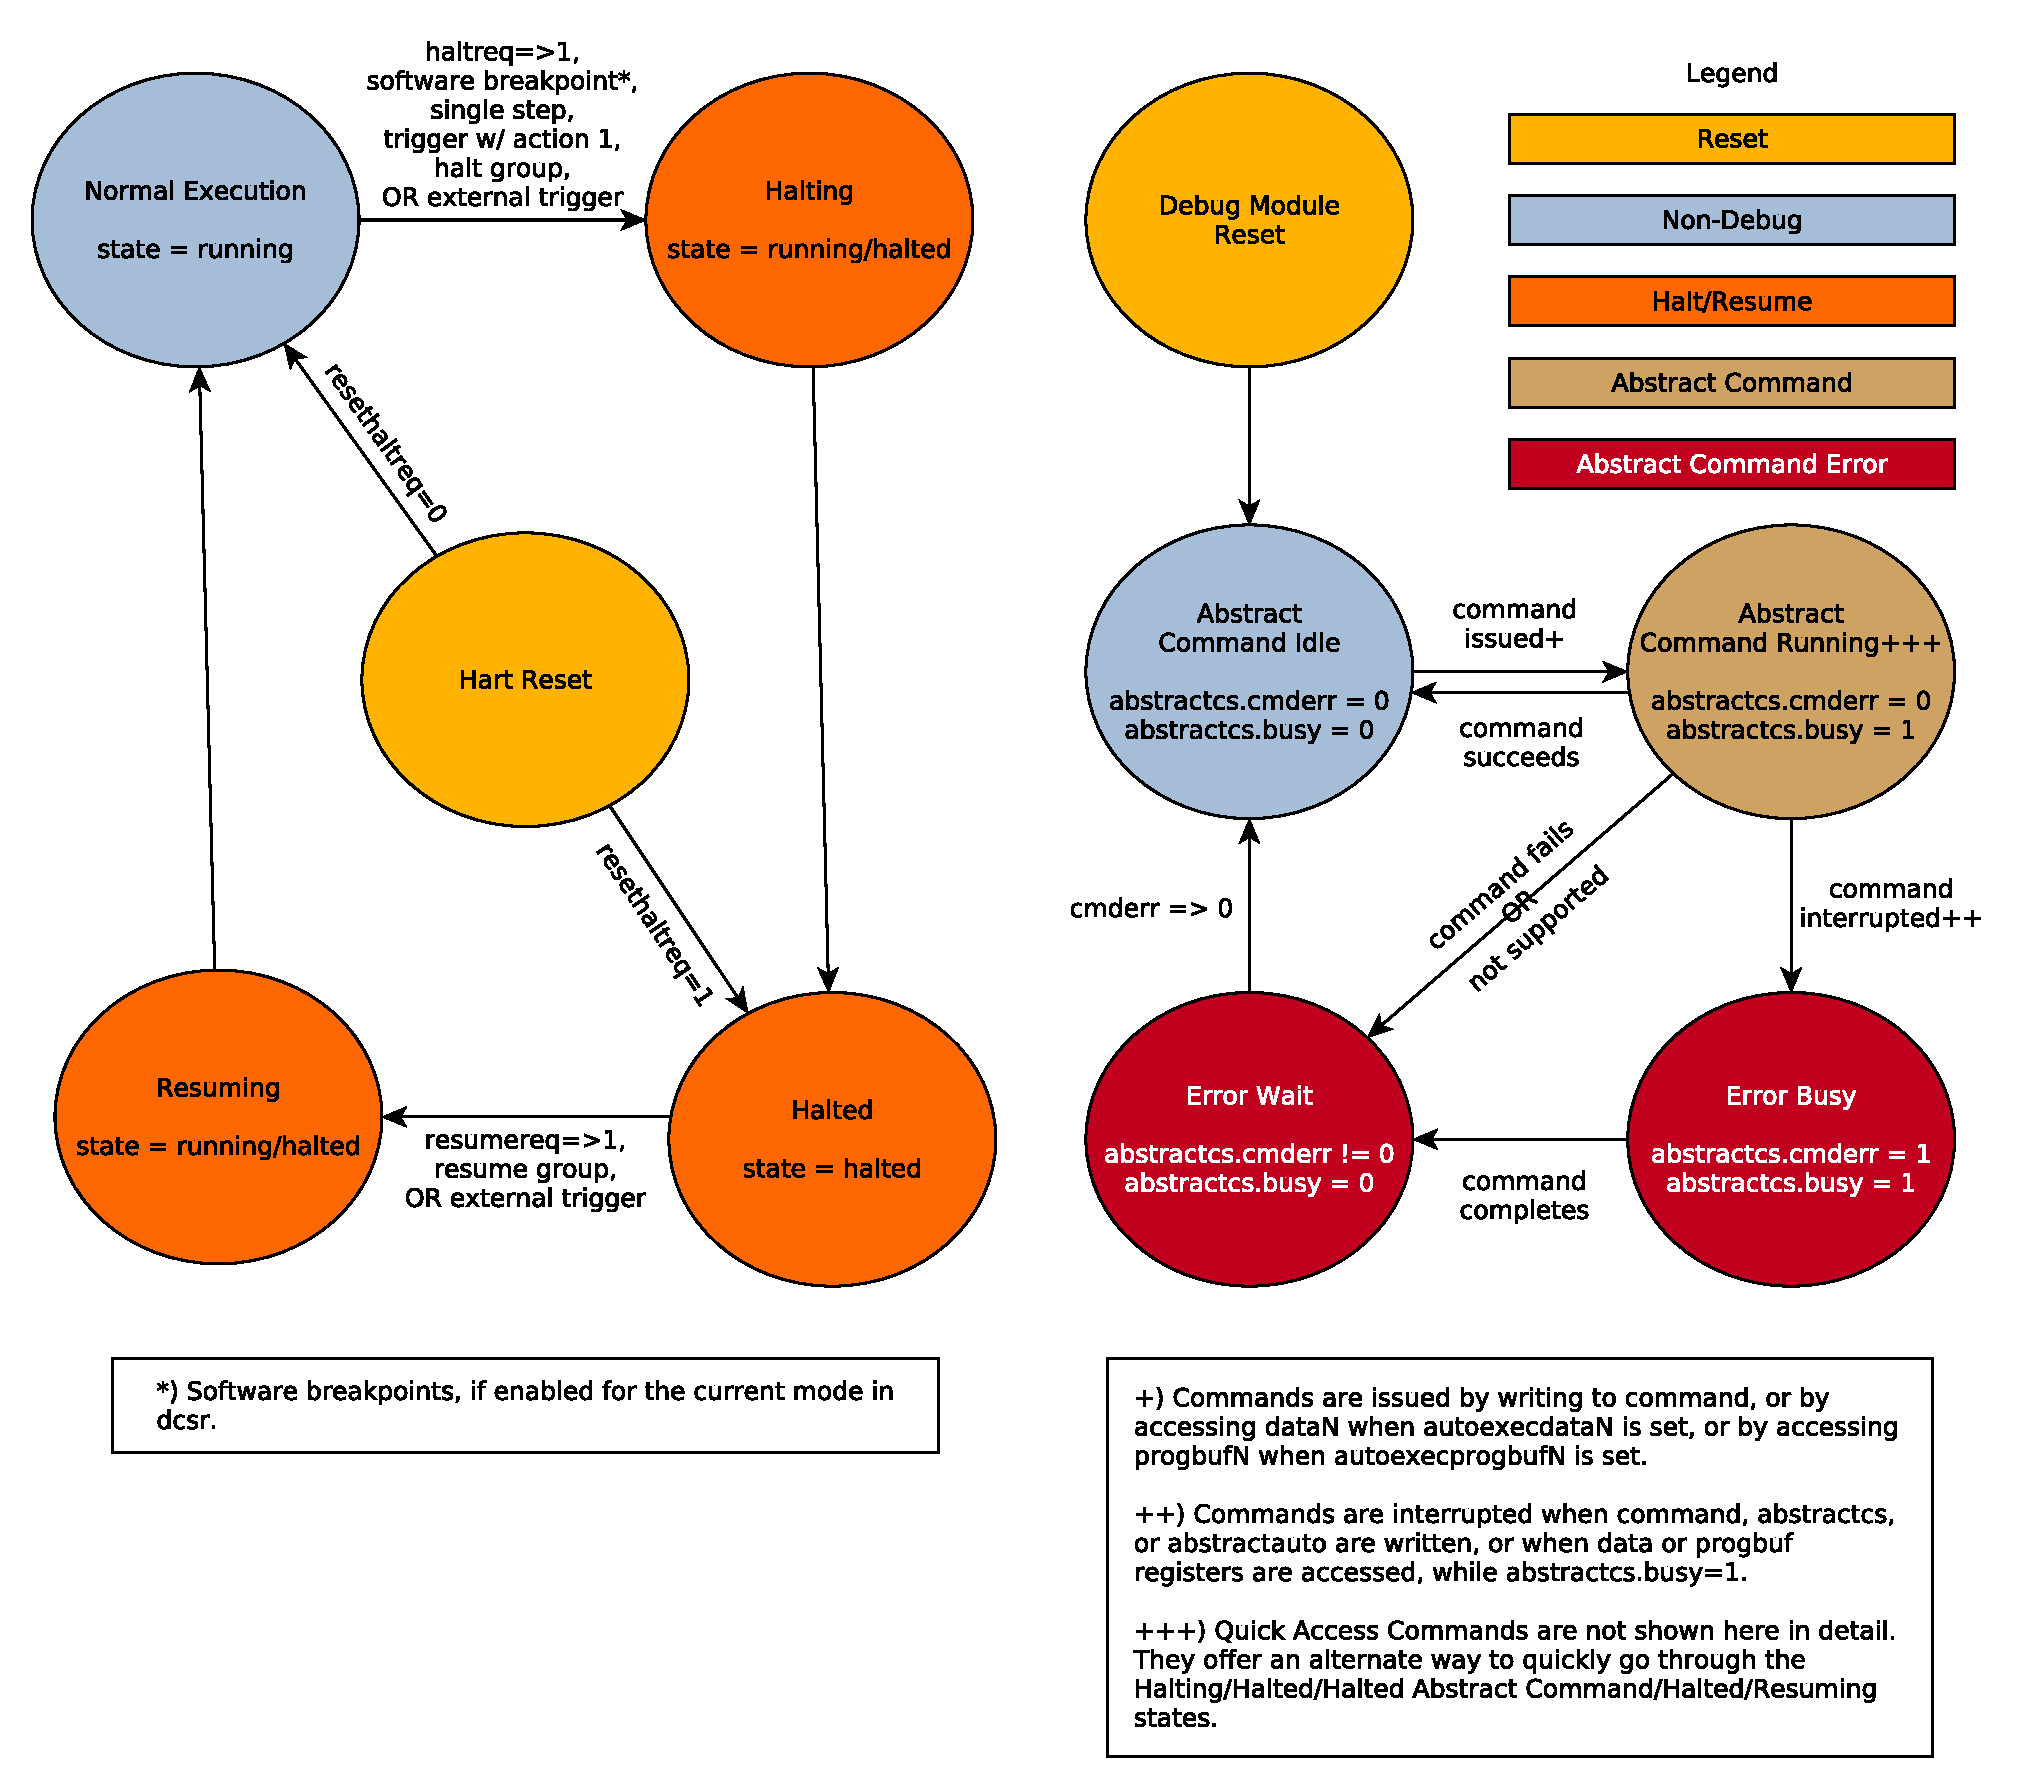
\includegraphics[width=\textwidth]{fig/abstract_commands.pdf}
   \caption[Run/Halt Debug State Machine]{Run/Halt Debug State Machine for single-hart systems.
     As only a small amount of state is visibile to the debugger,
     the states and transitions are conceptual.}
   \label{fig:abstract_sm}
\end{figure}

\section{System Bus Access} \label{systembusaccess}

A debugger can access memory from a hart's point of view using a Program Buffer or
the Abstract Access Memory command. (Both these features are optional.)
A Debug Module may also include a System Bus Access block to provide memory
access without
involving a hart, regardless of whether Program Buffer is implemented.
The System Bus Access block uses physical addresses.

The System Bus Access block may support 8-, 16-, 32-, 64-, and 128-bit
accesses. Table~\ref{tab:sbdatabits} shows which bits in {\tt sbdata} are used
for each access size.

\begin{table}[htp]
    \centering
    \caption{System Bus Data Bits}
    \label{tab:sbdatabits}
    \begin{tabulary}{\textwidth}{|r|l|}
        \hline
        Access Size & Data Bits \\
        \hline
        8 & \Rsbdatazero bits 7:0 \\
        \hline
        16 & \Rsbdatazero bits 15:0 \\
        \hline
        32 & \Rsbdatazero \\
        \hline
        64 & \Rsbdataone, \Rsbdatazero \\
        \hline
        128 & \Rsbdatathree, \Rsbdatatwo, \Rsbdataone, \Rsbdatazero \\
        \hline
    \end{tabulary}
\end{table}

Depending on the microarchitecture, data accessed through System Bus Access may
not always be coherent with that observed by each hart. It is up to the
debugger to enforce coherency if the implementation does not. This
specification does not define a standard way to do this.
Possibilities may include
writing to special memory-mapped
locations, or executing special instructions via the Program Buffer.

\begin{commentary}
Implementing a System Bus Access block has several benefits even
when a Debug Module also implements a Program Buffer.
First, it is possible to
access memory in a running system with minimal impact.  Second, it may improve
performance when accessing memory.
Third, it may provide
access to devices that a hart does not have access to.
\end{commentary}

\section{Minimally Intrusive Debugging}

Depending on the task it is performing, some harts can only be halted very briefly.
There are several mechanisms that allow accessing resources in such a running system
with a minimal impact on the running hart.

First, an implementation may allow some abstract commands to execute without halting the hart.

Second, the Quick Access abstract command can be used to halt a hart, quickly
execute the contents of the Program Buffer, and let the hart run again.
Combined with instructions that allow Program Buffer code to access the
{\tt data} registers, as described in \ref{hartinfo}, this can be used to quickly
perform a memory or register access. For some systems this will be too
intrusive, but many systems that can't be halted can bear an occasional hiccup
of a hundred or less cycles.

Third, if the System Bus Access block is implemented, it can be used while a
hart is running to access system memory.

\section{Security}

To protect intellectual property it may be desirable to lock access to the
Debug Module.  To allow access during a manufacturing process and not
afterwards, a reasonable solution could be to add a fuse bit to the Debug
Module that can be used to be permanently disable it. Since this is technology
specific, it is not further addressed in this spec.

Another option is to allow the DM to be unlocked only by users who have an
access key. Between \Fauthenticated, \Fauthbusy, and \Rauthdata arbitrarily
complex authentication mechanism can be supported.  When \Fauthenticated is
clear, the DM must not interact with the rest of the platform, nor expose
details about the harts connected to the DM. All DM registers should read 0,
while writes should be ignored, with the following mandatory exceptions:
\begin{steps}{}
    \item \Fauthenticated in \Rdmstatus is readable.
    \item \Fauthbusy in \Rdmstatus is readable.
    \item \Fversion in \Rdmstatus is readable.
    \item \Fdmactive in \Rdmcontrol is readable and writable.
    \item \Rauthdata is readable and writable.
\end{steps}

\section{Version Detection}

\begin{steps}{To detect the version of the Debug Module with a minimum of side
    effects, use the following procedure:}
    \item Read \Rdmcontrol.
    \item Write \Rdmcontrol, preserving \Fhartreset, \Fhasel, \Fhartsello, and
        \Fhartselhi from the value that was read, setting \Fdmactive, and
        clearing all the other bits.
    \item Read \Rdmstatus, which contains \Fversion.
\end{steps}

\begin{steps}{This has the following unavoidable side effects:}
    \item \Fhaltreq is cleared, potentially preventing a halt request made by a
        previous debugger from taking effect.
    \item \Fresumereq is cleared, potentially preventing a resume request made
        by a previous debugger from taking effect.
    \item \Fndmreset is deasserted, releasing the system from reset if a
        previous debugger had set it.
    \item \Fdmactive is asserted, releasing the DM from reset. This in itself
        is not observable by any harts.
\end{steps}

This procedure is guaranteed to work in future versions of this spec.  The
meaning of the \Rdmcontrol bits where \Fhartreset, \Fhasel, \Fhartsello, and
\Fhartselhi currently reside might change, but preserving them will have no
side effects. Clearing the bits of \Rdmcontrol not explicitly mentioned here
will have no side effects beyond the ones mentioned above.

\section{Debug Module Registers} \label{dmdebbus}

The registers described in this section are accessed over the DMI bus.  Each DM
has a base address (which is 0 for the first DM). The register addresses below
are offsets from this base address.

When read, unimplemented Debug Module DMI Registers return 0. Writing them has
no effect.

For each register it is possible to determine that it is implemented by reading
it and getting a non-zero value (e.g.\ \Rsbcs), or by checking bits in another
register (e.g.\ \Fprogbufsize).

\input{dm_registers.tex}
